\documentclass[a4paper,twocolumn,12pt]{article}
\usepackage[left=1.5cm, right=1.5cm, top=2cm,bottom=2cm]{geometry}
\usepackage{amsmath, amssymb, amsfonts}
\usepackage{enumerate}
\usepackage{graphicx}
\usepackage{tikz}
\begin{document} 
\section*{Piape Matemática} 
 
\subsection*{Módulo I}
\subsection*{Exercícios Aula 02}
   
\paragraph*{1.} Para cada descrição abaixo, enumere os elementos dos conjuntos envolvidos e represente-os em diagramas de Venn.

\begin{enumerate}[a)]
\item  \(A\) é o conjunto dos números pares entre 1 e 20.
\item \(B\) é o conjunto dos números ímpares entre 1 e 20.
\item \(C\) é o conjunto dos números primos entre 1 e 20.
\item \(D\) é o conjunto dos números múltiplos de 3 entre 1 e 20.
\item \(E\) é o conjunto dos números múltiplos de 5 entre 1 e 20.
\item \(F\) é o conjunto dos números primos que são pares. 
\item \(G\) é o conjunto dos números múltiplos de 6 entre 1 e 20.
\end{enumerate}

\paragraph*{2.} Considerando os conjuntos da questão anterior, complete os itens abaixo utilizando os símbolos \(\in\) e \(\notin\), \(\subseteq\) e \(\not\subseteq\).

\medskip
\newcommand{\complete}{\underline{\hspace{7mm}} }

\begin{minipage}[t]{0.4\columnwidth}
  
\begin{enumerate}[a)]
  \item 5 \complete $A$
  \item 7 \complete $B$
  \item 2 \complete $C$
  \item 9 \complete $D$
  \item 8 \complete $E$
  \end{enumerate}
  
\end{minipage}\hfil\begin{minipage}[t]{0.3\columnwidth}

\begin{enumerate}[a)]
  \setcounter{enumi}{5}
  \item $B$ \complete $A$
  \item $D$ \complete $B$
  \item $F$ \complete $C$
  \item $G$ \complete $D$
  \item $G$ \complete $A$
  \end{enumerate}
  
\end{minipage}

\paragraph*{3.} Se o conjunto \(A\) está contido no conjunto \(B\) e \(B\) está contido em \(C\), qual
  relação podemos estabelecer entre \(A\) e \(C\)?
 Represente a descoberta acima usando notação simbólica e usando diagramas de Venn.


\paragraph{4.} Para os exercício que segue, considere os seguintes conjuntos:
\begin{align*}
P &= \{1,2,3,4,8\}\\
Q &=  \{2,4,6\}\\
R &= \{1,3,5\}
\end{align*}
%\[ P = \{1,2,3,4,8\}\] \[ Q =  \{2,4,6\}\] \[ R = \{1,3,5\}\]
Calcule o que se pede. Represente o resultado em notação de diagramas de Venn.

\medskip

\begin{minipage}[t]{0.45\columnwidth}
  \begin{enumerate}[a)]
    \item \(P\cup Q\)
    \item \(Q\cup R\)
    \item \(P\cup Q \cup R\)
    \item \(P\cap Q\)
    \item \(Q\cap R\)
  \end{enumerate}
\end{minipage}\begin{minipage}[t]{0.45\columnwidth}
  \begin{enumerate}[a)]
    \setcounter{enumi}{5}
    \item \(P\setminus Q\)
    \item \(Q\setminus P\)
    \item \(P\setminus R\)
    \item \(R\cap P\)
  \end{enumerate}
\end{minipage} 

\paragraph{5.} Calcule os tamanhos dos conjuntos
\begin{enumerate}[a)]
  \item \(|P\cup Q|\)
  \item \(|P\cap Q|\)
  \item \(|Q\cup R|\)
  \item \(|Q\cap R|\)
\end{enumerate}

\paragraph{6.} Essa é uma questão mais teórica. Considere $X$ e $Y$ conjuntos quaisquer. 
\begin{enumerate}[a)] 
\item Qual relação de inclusão entre os conjuntos \(X\), \(Y\) e \(X\cup Y\)?
\item Qual relação de inclusão entre os conjuntos \(X\), \(Y\) e \(X\cap Y\)?
\end{enumerate}

 

\vspace*{\fill}

{\footnotesize \color{darkgray}
\paragraph*{Gabarito} \hspace*{\fill}\\
\textbf{1.} a) A = \{2, 4, 6, 8, 10, 12, 14, 16, 18, 20\}; b) B = \{1, 3, 5, 7, 9, 11, 13, 15, 17, 19\}; c) C = \{2, 3, 5, 7, 11, 13, 17, 19\}; d) D = \{3, 6, 9, 12, 15, 18\}; e) E = \{5, 10, 15, 20\}; f) F = \{2\}; g) G = \{6, 12 ,18\}\\
\textbf{2.} a) \(5\notin A\); b) \(7\in B\); c) \(2\in C\); d) \(9\in D\); e) \(8\notin E\); f) \(B\not\subseteq A\); g) \(D\not\subseteq B\); h) \(F\subseteq C\); i) \(G\subseteq D\); j) \(G\subseteq A\)\\
\textbf{3.} a) \(A \subseteq C\); b) 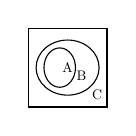
\begin{tikzpicture}[scale=0.5, every node/.style={scale=0.5}]
  \draw (-0.2,0) ellipse (0.4cm and 0.5cm);
  \node at (0,0) {A};  

  \draw (0,0) ellipse (0.8cm and 0.7cm);
  \node[left] at (0.6,-0.2) {B};
  
  \draw (-1,-1) rectangle (1,1);
  \node[left] at (1,-0.7) {C};
\end{tikzpicture}\\
\textbf{4.} a) \(P\cup Q = \{1,2,3,4,6,8\}\); b) \(Q\cup R = \{1,2,3,4,5,6\}\); c) \(P\cup Q \cup R = \{1,2,3,4,5,6,8\}\); d) \(P\cap Q = \{2,4\}\); e) \(Q\cap R = \emptyset\); f) \(P\setminus Q = \{1,3,8\}\); g) \(Q\setminus P = \{6\}\); h) \(P\setminus R = \{2,4,8\}\); i) \(R\cap P = \{1,3\}\)\\
\textbf{5.} a) \(|P\cup Q| = 6\); b) \(|P\cap Q| = 2\); c) \(|Q\cup R| = 6\); d) \(|Q\cap R| = 0\)\\
\textbf{6.} a) \(X\subseteq X\cup Y\) e também $Y\subseteq X\cup Y$; b) \(X\cap Y\subseteq X\) e também \(X\cap Y\subseteq Y\)

}


\end{document}